\documentclass[a4paper]{article}
%\usepackage{vntex}
%\usepackage[english,vietnam]{babel}
\usepackage[utf8]{vietnam}

\usepackage{multirow} %enable mutirow
\usepackage{array} % enable us to define new content format in table
\newcolumntype{P}[1]{>{\centering\arraybackslash}p{#1}}
\newcolumntype{M}[1]{>{\centering\arraybackslash}m{#1}}

\usepackage[linesnumbered,lined,ruled,commentsnumbered]{algorithm2e}

\makeatletter
\def\BState{\State\hskip-\ALG@thistlm}
\makeatother

\usepackage{a4wide,amssymb,epsfig,latexsym,multicol,array,hhline,fancyhdr}
\usepackage{float}
\restylefloat{table}
\usepackage{amsmath}
\usepackage{lastpage}
%\usepackage[lined,boxed,commentsnumbered]{algorithm2e}
\usepackage{enumerate}
\usepackage{color}
\usepackage{graphicx}							% Standard graphics package
\usepackage{array}
\usepackage{tabularx, caption}
\usepackage{multirow}
\usepackage{multicol}
\usepackage{rotating}
\usepackage{graphics}
\usepackage{geometry}
\usepackage{setspace}
\usepackage{epsfig}
\usepackage{booktabs}% http://ctan.org/pkg/booktabs
\newcommand{\tabitem}{~~\llap{\textbullet}~~}
\usepackage{tikz}
\usetikzlibrary{arrows,snakes,backgrounds}
\usepackage{hyperref}
\hypersetup{urlcolor=blue,linkcolor=black,citecolor=black,colorlinks=true} 
%\usepackage{pstcol} 								% PSTricks with the standard color package

\newcommand{\matr}[1]{\mathbf{#1}}
\renewcommand{\vec}[1]{\mathbf{#1}}
\newcommand{\code}[1]{\texttt{#1}}
\DeclareMathOperator*{\argmax}{\arg\!\max}
\renewcommand*\descriptionlabel[1]{\hspace\leftmargin$#1$}
%\DeclarePairedDelimiter\abs{\lvert}{\rvert}
\usepackage{siunitx}
\relpenalty=10000
\binoppenalty=10000
\usepackage{listings}

\usepackage{fancyhdr}
\setlength{\headheight}{40pt}
\pagestyle{fancy}
\fancyhead{} % clear all header fields
\fancyhead[L]{
 \begin{tabular}{rl}
    \begin{picture}(25,15)(0,0)
    \put(0,-8){
\includegraphics[width=8mm, height=8mm]{hcmut.png}}
    %\put(0,-8){\epsfig{width=10mm,figure=hcmut.eps}}
   \end{picture}&
	%
\includegraphics[width=8mm, height=8mm]{hcmut.png} & %
	\begin{tabular}{l}
		\textbf{\bf \ttfamily Ho Chi Minh University of Technology}\\
		\textbf{\bf \ttfamily Department of Computer Science and Engineering}
	\end{tabular} 	
 \end{tabular}
}
\fancyhead[R]{
	\begin{tabular}{l}
		\tiny \bf \\
		\tiny \bf 
	\end{tabular}  }
\fancyfoot{} % clear all footer fields
\fancyfoot[L]{\scriptsize \ttfamily Assignment for Computer Architecture - Year 2019 - 2020}
\fancyfoot[R]{\scriptsize \ttfamily Page {\thepage}/\pageref{LastPage}}
\renewcommand{\headrulewidth}{0.3pt}
\renewcommand{\footrulewidth}{0.3pt}


%%%
\setcounter{secnumdepth}{4}
\setcounter{tocdepth}{3}
\makeatletter
\newcounter {subsubsubsection}[subsubsection]
\renewcommand\thesubsubsubsection{\thesubsubsection .\@alph\c@subsubsubsection}
\newcommand\subsubsubsection{\@startsection{subsubsubsection}{4}{\z@}%
                                     {-3.25ex\@plus -1ex \@minus -.2ex}%
                                     {1.5ex \@plus .2ex}%
                                     {\normalfont\normalsize\bfseries}}
\newcommand*\l@subsubsubsection{\@dottedtocline{3}{10.0em}{4.1em}}
\newcommand*{\subsubsubsectionmark}[1]{}
\makeatother


\begin{document}

\begin{titlepage}
\begin{center}
VIET NAM NATIONAL UNIVERSITY, HO CHI MINH CITY \\
HO CHI MINH UNIVERSITY OF TECHNOLOGY\\
DEPARTMENT OF COMPUTER SCIENCE AND ENGINEERING 
\end{center}

\vspace{1cm}

\begin{figure}[h!]
\begin{center}

\includegraphics[width=3cm]{hcmut.png}
\end{center}
\end{figure}

\vspace{1cm}


\begin{center}
\begin{tabular}{c}
\multicolumn{1}{l}{\textbf{{\Large COMPUTER ARCHITECTURE}}}\\
~~\\
\hline
\\
\multicolumn{1}{l}{\textbf{{\Large MAR MIPS Assignment}}}\\
\\
\textbf{{\Huge Sorting and Searching on Array}}\\
\\
\hline
\end{tabular}
\end{center}

\vspace{3cm}

\begin{table}[h]
\begin{tabular}{rrl}
\hspace{5 cm} & Instructor: & Phạm Quốc Cường\\
& Student: & Trần Hoàng Long - 1852545 \\
\end{tabular}
\end{table}

\begin{center}
{\footnotesize Ho Chi Minh City, Dec 2019}
\end{center}
\end{titlepage}


%\thispagestyle{empty}

\newpage
\tableofcontents
\newpage
\section{Introduction}
This paper summarizes my research, notes and implementation on the Computer Architecture MIPS Assignment.
There are two exercises:
\begin{itemize}
\item Implement QuickSort in MIPS, sort an array decendingly and report it's instruction count, execution time (assuming $1ns$ each instruction)
\item Implement BinarySearch in MISP. First, sort an array assendingly and then use QuickSort implemented to find \emph{all indexes} of an element.
\end{itemize}
For exercise 1, i will show my algorithms and ideas. To calculate the execution, i would analyze my algorithm and test my program in different cases: Worst, Best and Average.\\
For exercises 2, i will show the original BinarySearch, then explan my modifications to get BinarySearch working with duplicated elements and then show my implementation with a test example.\\
There's another section in the end where i show some notes and ideas i came accross while working with MIPS for the project, as well as reviewing my implementation for the exercises from the "MIPS" perspective.
\section{Exercise 1}
\subsection{Quick Sort Algorithm}
Quick sort algorithm is highly efficient sorting algorithm. It's based on:
\begin{enumerate}
\item Piking an item as a pivot (many different ways pivot can be chosen) but in my implementation, i always pick pivot as array's last element
\item Partitioning the array into two smaller sub-arrays around pivot, one half is larger and the other is smaller than pivot. Thus putting pivot at the correct position.
\item Then, recursively call the Quick sort function again to sort the sub-arrays until all are sorted.
\end{enumerate}
\begin{algorithm}[H]
\DontPrintSemicolon
\SetAlgoLined
  \KwIn{$head$ and $tail$ address of array}
  \KwOut{Void}
  \KwResult{Array from $head$ to $tail$ sorted}
	\BlankLine  
  \Begin{
    \If{$(head < tail)$}{
      $pivot = Partition(head,tail)$\;
      $QuickSort (head,pivot-1)$\;
		$QuickSort (pivot+1,tail)$\;
    }
    }
  \caption{QuickSort}
\end{algorithm}
The function $Partition(head,tail)$ takes two arguments: the head address and tail address of the array, it spit the array into two halves one on the left is larger and the right is smaller than pivot \emph{(since we are sorting in decending order)}. After partitioning, it reposition the pivot in the middle of the two sub-sets and return the new address of pivot.\\
\begin{algorithm}[H]
\DontPrintSemicolon
\SetAlgoLined
  \KwIn{$head$ and $tail$ address of array}
  \KwOut{New correct address of $pivot$}
  \KwResult{Array partition into two halves with pivot in the middle}
	\BlankLine  
  \Begin{
  $pivot = tail$ \;
    \While{$(1)$}{
    	\While{$(head.Value>pivot.Value)$}{
    	$head++$\;
    	}
    	\BlankLine  
    	\While{$(tail.Value\leqslant pivot.Value) \&\& (tail>head)$}{
    	$tail--$\;
    	}
    	\BlankLine  
    	\eIf{$(head<tail)$}
    	{
    	$Swap(head.Value,tail.Value)$\;
    	}{
    	\textbf{break}\;
    	}
    	
    }
    $Swap(pivot.Value,head.Value)$\;
    \Return{$head$}
    }
  \caption{Partition}
\end{algorithm}

In the partition algorithm, we constantly check the value to the left and the right of the array and move inward to continue checking, if we find a pair of value in the incorrect position, we swap them. After this, we swap the pivot into the middle of two partitions and return it's new address.
\subsection{Complexity}
\subsubsection{Best-case analysis}
In the most balanced case, each time we perform a partition we divide the list into two nearly equal pieces. This means each recursive call processes a list of half the size. Each of the sub-set can only be equal or within one of each other in this case.\\
In this case, complexity is same as Merge Sort, $O(n\log_2{n})$
\begin{center}
    \begin{figure}[H]
    \begin{center}
     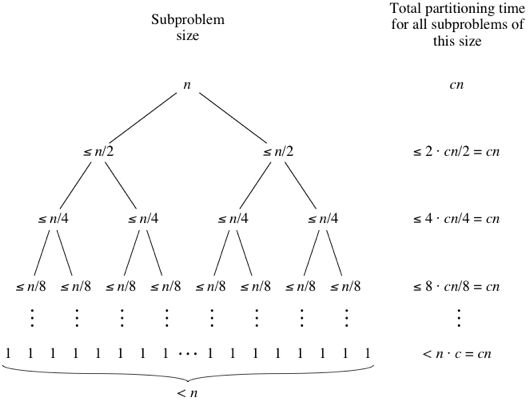
\includegraphics[scale=1.2]{Quick_best}
    \end{center}
    \caption{Tree of best case sub-problem sizes}
    \label{ref0}
    \end{figure}
\end{center}
\subsubsection{Worst-case analysis}
The most unbalanced case occurs when the recursive call on the $i^{th}$ element takes $i-1$ time. $(i\in\{n,n-1,...,0\})$
\begin{center}
    \begin{figure}[H]
    \begin{center}
     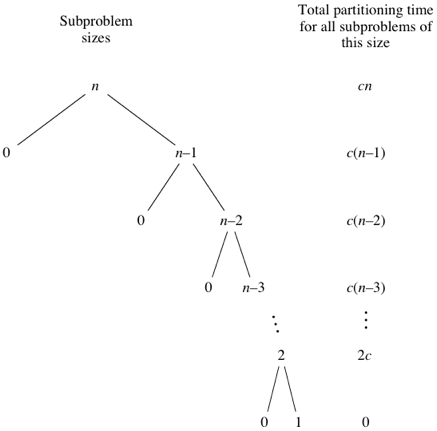
\includegraphics[scale=1.2]{Quick_worst}
    \end{center}
    \caption{Tree of worst case sub-problem sizes}
    \label{refhinh1}
    \end{figure}
\end{center}
If this happens repeatedly in every partition, then each recursive call processes a list of size one less than the previous list. And in that case, Quicksort takes $O(n^2)$ time.
\subsubsection{Average-case analysis}
In the average case, the complexity is $O(n\log_2{n})$.
\begin{center}
    \begin{figure}[H]
    \begin{center}
     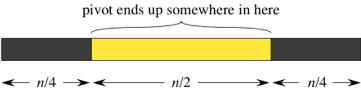
\includegraphics[scale=1.2]{Quick_ave}
    \end{center}
    \caption{Tree of best case sub-problem sizes}
    \label{ref0}
    \end{figure}
\end{center}
\subsection{Execution time example}
Knowing the diffrent cases of complexity of QuickSort, i've tested my implementation to see the instruction count and execution time. \emph{Assuming that all the instructions executes equally, requiring \textbf{1 ns} of processing.}
I tested by running the program on some random sorted array of different sizes (dupplication allowed). (Generated through \url{https://www.calculatorsoup.com} and \url{https://www.random.org})\\
Instructions are counted using the Instruction Counter intergrated in MARS 4.5.
\subsubsection{Worst Case Performance}
In my implementation, the pivot is chosen as the last element, so it's easy to see that the worst case will be when our array is already sorted. If this happens, the partition function will only process one element each time and the worst case senario happens.\\
\textbf{Test: }
\begin{table}[H]
\centering
\begin{tabular}{|P{2cm}|P{2cm}P{2cm}|P{2cm}P{2cm}P{2cm}P{2cm}|}
\hline
\multirow{2}{*}{No.} & \multirow{2}{*}{Array} & \multirow{2}{*}{Size} & \multicolumn{4}{c|}{Instruction} \\
\cline{4-7}
 &  &  & I-Type & R-Type & J-Type & Total \\
\hline
1	&$X \in [1,100]$&	10&	542&	267&	68&	877\\	
2	&$X \in [1,1000]$&	100&	21332&	14037&	5198&	40567\\
3	&$X \in [1,10000]$&	1000&	1788482&	1265487&	501998&	3555967\\
4	&$X \in [1,100000]$&	10000&	175384982&	125154987&	50019998&	350559967\\
\hline
\end{tabular}
\caption{Instruction count for sorted random generated arrays}
\label{Bảng 1}
\end{table}
Given, theoretically, one instruction takes \textbf{1 ns}, the tested cases above would take:
$877 ns$, $40.567\mu s$, $3.556ms$ and $0.35s$ respectively\\
But, in realtime, when simulating the worst case for the array of size 10000 elements, my code took real long too finish (a few hours), so i would take this as the limit for the worst case implementation.\\
The arrays used here are located in this \href{./Test_Array/Worst_sort.txt}{DataFile}
\subsubsection{Best and Average Case Performance}
Sometimes, the Partition function will split the array into two perfect half, and when this happens for all recursive calls of QuickSort, we get the best case scenario, if not, we would usually get the average case for QuickSort.\\
\textbf{Test: }I will test my implementation on random, unordered arrays (dupplication allowed).
\begin{table}[H]
\centering
\begin{tabular}{|P{2cm}|P{2cm}P{2cm}|P{2cm}P{2cm}P{2cm}P{2cm}|}
\hline
\multirow{2}{*}{No.} & \multirow{2}{*}{Array} & \multirow{2}{*}{Size} & \multicolumn{4}{c|}{Instruction} \\
\cline{4-7}
 &  &  & I-Type & R-Type & J-Type & Total \\
\hline
1	&$X \in [1,100]$&	10&	434&	217&	51&	702\\	
2	&$X \in [1,1000]$&	100&	5657&	3266&	868&	9791 \\
3	&$X \in [1,10000]$&	1000&	82358&	48021&	15723&	146102 \\
4	&$X \in [1,10000]$&	10000&	988861&	637136&	188500&	1814497 \\
5	&$X \in [1,100000]$&	100000&	12582457&	8214842&	2581215&	23378514 \\
\hline
\end{tabular}
\caption{Instruction count for random generated arrays}
\label{Bảng 1}
\end{table}
Given, theoretically, one instruction takes \textbf{1 ns}, the tested cases above would take:
$702 ns$, $9.791\mu s$, $0.1461ms$, $1.815ms$ and $0.0234s$ respectively\\
Diffrent from the worst case, my implementation can get to much better array size in random situation, up to 100000 element and might be more.
The arrays used here are located in this \href{./Test_Array/BestAv_sort.txt}{DataFile}
\section{Exercise 2}
\subsection{Binary Search}
Binary Search is searching a sorted array by repeatedly dividing the search interval in half. Begin with an interval covering the whole array. If the value of the search key is less than the item in the middle of the interval, narrow the interval to the lower half. Otherwise narrow it to the upper half. Repeatedly check until the value is found or the interval is empty.\\
\begin{algorithm}[H]
\DontPrintSemicolon
\SetAlgoLined
  \KwIn{$head$ and $tail$ address of array, search\_value to find in array}
  \KwOut{Address of searched value, $NULL(0x00000000)$ if not found}
	\BlankLine  
  \Begin{
  $mid = head + (tail-head)/2$\;
    \uIf{$(mid.Value == search\_value)$}{
      \Return{mid}\; 	
    }\uElseIf{$search\_value< mid.Value$}
    {$BinarySearch(head, mid-1)$}
    \Else{$BinarySearch(mid+1, tail)$}
    }
  \caption{Binary Search}
\end{algorithm}
That, was the key concept of binary search, but, in order to search and display all the occurrences of an element in the array, i made some adjustments. Here, i would search for the first occurence and if that exists in the array, continue to search for last occurence and print all indexes between, else, print $-1$.\\\\
\begin{algorithm}[H]
\DontPrintSemicolon
\SetAlgoLined
  \KwIn{$head$ and $tail$ address of array, $search\_value$ to find in array}
  \KwResult{All indexes of $search\_value$ printed, separated by "space" character, print $-1$ if none is found}
	\BlankLine  
  \Begin{
  		$first\_occur = BinarySearchFirst(head,tail,search\_value)$\;
  		\BlankLine  
  		\eIf{$firsr\_occur \neq NULL$}{
  		\BlankLine  
  		$last\_occur = BinarySearchLast(head,tail,search\_value)$\;
  		\BlankLine 
  		\While{$first\_occur\leqslant last\_occur$}{
			$print(first\_occur - head)$\;
			  		$first\_occur++$\;
  		}
		}{
		$print(-1)$
		}
    }
  \caption{Binary Search Print (all occurences)}
\end{algorithm}
For the BinarySearchFirst and BinarySearchLast, they're the same as normal binary search, but, instead of returning the address of value when found, they store the found address and keep searching to the left (Search First case) or to the right (Search Last case) and return the address later at the end.\\
\begin{algorithm}[H]
\DontPrintSemicolon
\SetAlgoLined
  \KwIn{$head$ and $tail$ address of array, $search\_value$ to find in array}
  \KwOut{Address of first OR last occurence of $search\_value$. $NULL$ if not found}
	\BlankLine  
  \Begin{
  		$first$ OR $last = NULL$\emph{  \textbf{// initial found address is NULL}}\;
  		\While{$head \leqslant tail$}
  		{
  			$middle = head + (tail-head)/2$\;
  			\uIf{$middle.Value$ == $search\_value$}
  			{ 
  				$first$ OR $last = middle$ \emph{  \textbf{//if found, save address}}\;
  				\BlankLine
  				\emph{\textbf{  //if looking for first, keep search left; if last, search right.}}\;
  				$tail = middle -1$ \textbf{OR} $head = middle +1$
  			}\uElseIf{$search\_value < middle.Value$}
  			{ 
  				$tail = middle -1$\;
  			}\Else
  			{
  				$head = middle +1$\;
  			}
  		}
  		
  		\Return {$first$ OR $last$}
    }
  \caption{Binary Search First OR Last}
\end{algorithm}
\subsection{Example}
Assume an array as follows:
\begin{center}
$10, 5, 1, 3, 10, 7, 1, 3, 1, 2, 3, 7, 7, 1, 8, 10, 3, 2, 1, 10$
\end{center}

\textbf{My implementation's procedure is as follows:}
\begin{enumerate}
\item  Print initial array 
\item Sort ascendingly using QuickSort
\item Ask for user input for element to search for binarily
\item Display all found indexes
\end{enumerate}
\begin{center}
    \begin{figure}[H]
    \begin{center}
     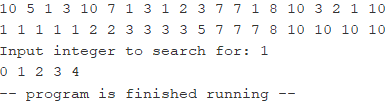
\includegraphics[scale=1.2]{BinSearchEx.png}
    \end{center}
    \caption{MIPS output for searching element 1}
    \label{refhinh1}
    \end{figure}
\end{center}

Note that the BinarySearch implemented by me does not actually store the found indexes in any way, but instead, find the first, last address and print all indexes.
\section{MIPS Implementation Notes and Ideas}
\subsection{Calling Convention}
As known, CPU only have a handful of register for us to work with on all of our functions, and it's possible for different function to use same registers, leading to overwriting and corruption during callling process. This leads us to the use of stack to save/restore register value to help preserve our registers. The conventional use of this is described briefly below:
\begin{enumerate}
\item Argument registers $\$a$ are usually copied into other registers for usage. If function want to moddfy directly, must be pushed to stack before use and restored later.
\item Temporary $\$s$ registers are expected to be unchanged in a function call, so the callee must save/restore them if need for usage.
\item Temporaty $\$t$ registers are seen as "could be changed", so the caller need to save them before making a function call (restore after call) and the callee does not care when using them.
\item The return address $\$ra$ register is always saved and restore if the function is not a leaf (means it calls others at some point)
\end{enumerate}
\textbf{Note:} Careful when designing a function that's a caller and also a callee.\\
When coding the recursive function QuickSort in the assignment, it's important to notice that it is a caller as well as a callee, so all register modified must be saved, including the $\$ra$ register.
\subsection{Implement MIPS QuickSort}
My implementation of QuickSort in MIPS is rather simple:
\begin{enumerate}
\item Print the array one before sorting
\item Call the QuickSort (decending) function:
	\begin{itemize}
	\item Argument is $\$a1$ and $\$a2$ as head and tail address of array
	\item Pivot is always the element at the tail
	\item Call the Partition function (also take argument $\$a1$ and $\$a2$ as head and tail to of array) to sort the array into to halves and put the pivot in the middle, returning new address of pivot.
	\item Continue to sort on the two sides of the new location of pivot until all sorted.
	\end{itemize}
\item Print the array after sorting
\end{enumerate}
\subsection{Implement MIPS BinarySearch}
For exercise 2, it's required to sort and binarily search for all indexes of a value.\\
First, i sort the given array using QuickSort that i've already implemented (but asscending this time).\\
And then initialize BinarySearch (dupplicated element allowed):
\begin{enumerate}
\item BinarySearch calls for BinarySeachFirst and BinarySearchLast (all three functions take arguments: $\$a1 - head$,$\$a2 - tail$ and $\$a3 - search\_value$)
\item BinarySearchFirst/Last would find the \textbf{address} of first/last occurence of element using BinarySeachAlgorithm (modified) and return it in $\$v1$
\item After getting the first and last address, BinarySearch will translate the address into the element's relative index to the head of array and print all index between.
\item Case element not found, the return address from BinarySearchFirst is $NULL$, and BinarySeach would print $-1$ instead.
\item Note that i don't store the found index in anyway but instead only get the first,last address, then translate them and print all index got.
\end{enumerate}
\end{document}